\documentclass[12pt,oneside]{book}

\title{Application for Promotion to Candidacy}
\author{File Preparation Committee}
\date{2024}

\usepackage[T1]{fontenc}

% Specify the font.
\usepackage{fourier} % Adobe Utopia

% For better formatting in the table listing referees
\usepackage{array}

% Page margins.
\usepackage[margin=2cm]{geometry}

\setlength{\headheight}{15pt}

\usepackage{microtype}
\microtypecontext{spacing=nonfrench}

% Say "A", not "Chapter A", by removing the word \chapter.
\renewcommand{\chaptername}{}

% Candidate's notes
\newcommand*{\notefont}{\fontfamily{phv}\selectfont}

% To include images
% \usepackage{graphicx}

% Tighter lists.
\usepackage{enumitem}
\setlist{noitemsep}

% For rules in tables
\usepackage{booktabs}

% For better formatting in the table listing referees
\usepackage{array}

% To allow H location for image floating (meaning "right here")
\usepackage{float}

% Figures float, but minipages don't, so these let me
% me put graphics where I want, labelled, with captions.
% \usepackage{wrapfig}
% \usepackage{caption}

% To include other PDFs. Section and page numbering are all handled perfectly.
\usepackage{pdfpages}
% When including slides do this to make a 2x3 layout:
% \includepdf[pages=-,nup=2x3,delta=5mm 5mm,landscape=false]{filename.pdf}

% I was getting errors like this:
% pdfTeX warning: pdflatex (file ./2-4-1-lrts-frbr-book-review.pdf): PDF inclusion: found PDF version <1.7>, but at most version <1.5> allowed
% but this fixes it:
\pdfoptionpdfminorversion=7

% Suppress warnings like this:
% pdfTeX warning: pdflatex (file ./pdfs/B 2.2.1 Introduction to Data Visualization for Research.pdf): PDF inclusion: multiple pdfs with page group included in a single page
\pdfsuppresswarningpagegroup=1

% For better table formatting
%\usepackage{multirow}
%\usepackage{rotating}
%\usepackage{longtable}

% Start numbering sections at 0.  Because that's where numbering starts.
% \setcounter{section}{-1}
% \setcounter{chapter}{-1}

% Nice headers.
\usepackage{fancyhdr}
\pagestyle{fancy}
\fancyhf{}
%  \thepage, \thesubsection etc.  \leftmark is chapter title, \rightmark is section title
% \renewcommand{\headrulewidth}{1pt}

\newcommand{\chaptertitle}{}
\renewcommand{\chaptermark}[1]{\renewcommand{\chaptertitle}{Chapter \thechapter\ #1}}
\renewcommand{\sectionmark}[1]{\markboth{\thesection\ #1}{}}
\renewcommand{\subsectionmark}[1]{\markright{\thesubsection\ #1}}

% Colours red the line above the footer.
\renewcommand{\footrule}{\hbox to\headwidth{\color{red}\leaders\hrule height \headrulewidth\hfill}}

% Turn \url and \href into hyperlinks in PDFs, and pass hyphens option to url package
% (which hyperref calls) to get better line breaks.
% http://tex.stackexchange.com/questions/3033/forcing-linebreaks-in-url?rq=1
\PassOptionsToPackage{hyphens}{url}\usepackage[pdfborder={0 0 0},colorlinks=true,urlcolor=blue]{hyperref}

% With this I can say \link{https://example.com/} and it makes it a hyperlink wrapped in < >
\newcommand{\link}[1]{{\small $<$\url{#1}$>$}}

% Add PDF properties (part of hyperref)
\hypersetup{%
  bookmarksnumbered, % To get A 1.2 etc. into the bookmarks
  pdfauthor={File Preparation Committee},
  pdfsubject={},
  pdftitle={Letters of Reference},
  pdfkeywords={},
  linkcolor=black % Other TOC listings, and internal links, are in red
}

% \attached puts a short horizontal rule, with some space above and below,
% which I'll follow with a list of the attachments for the section.
\newcommand{\attached}{%
\vspace{1em}
\noindent\rule{8cm}{0.4pt}
\newline
\vspace{1em} Attached:
}

% No paragraph indent.
% \setlength{\parindent}{0pt}
% \setlength{\parskip}{\baselineskip}

% Remove the page numbers from the TOC.
% \let\Contentsline\contentsline
% \renewcommand\contentsline[3]{\Contentsline{#1}{#2}{}}


% DRAFT: comment this out when it's not a draft.
% \usepackage[firstpageonly=true,scale=1.5]{draftwatermark}

% Footers: Put the last name in both these places.
% The rest of the footer is configured in common-latex.tex.
\fancyfoot[L]{Name}

\fancypagestyle{plain}{%
  \fancyfoot[L]{Name}
}

% Start numbering sections at 0.  You can leave this alone.
\setcounter{section}{-1}
\setcounter{chapter}{-1}

\begin{document}

\frontmatter

\begin{titlepage}

  \null\vfill

  \begin{center}

    {\Huge
      Application for Advancement/Promotion
    }
    \vspace{2cm}

    {\Large
      Name Here
    }
    \vspace{1cm}

  {\large
    Position Title

    York University Libraries

    \vspace{1cm}

    dd Month 2024

  }

\end{center}

\vfill
\vfill

{\large
  File Preparation Committee:

  Name One (Associate Librarian), chair \\
  \indent Name Two (Associate Librarian) \\
  \indent Name Three (Associate Librarian)
}

\hfill

\end{titlepage}

% \begin{abstract}
% ...
% \end{abstract}

% \listoffigures

\tableofcontents

% Suppress CONTENTS in footer of table of contents
\markboth{}{}

\mainmatter{}

\chapter{Front matter}

\pagenumbering{arabic}

\section{Curriculum vit\ae}

\begin{itemize}
  \item Current CV.\@  The included PDF is shrunk to 95\% of its original size.
\end{itemize}


\includepdf[pages=-,scale=0.95,pagecommand={}]{pdfs/example-2.pdf}

\section{Job description}

\begin{itemize}
  \item Job description (2023)
\end{itemize}


\includepdf[pages=-,scale=0.95,pagecommand={}]{pdfs/example-1.pdf}

\section{Personal statement}

\begin{itemize}
  \item Personal statement from the candidate
\end{itemize}


\includepdf[pages=-,scale=1,pagecommand={}]{pdfs/example-2.pdf}

\renewcommand\thechapter{A}
\chapter{Professional Performance and Knowledge}
% \label{chapter:ppk}

\section{Teaching}

\subsection{Course name}

\begin{itemize}
  \item Included slides (showing that multiple slides can be shown on one page; the arrangement is easily configurable).
\end{itemize}

\candidatenote{
  This is a note from the candidate.  It has a different typeface and stands out from the rest of the file.
}

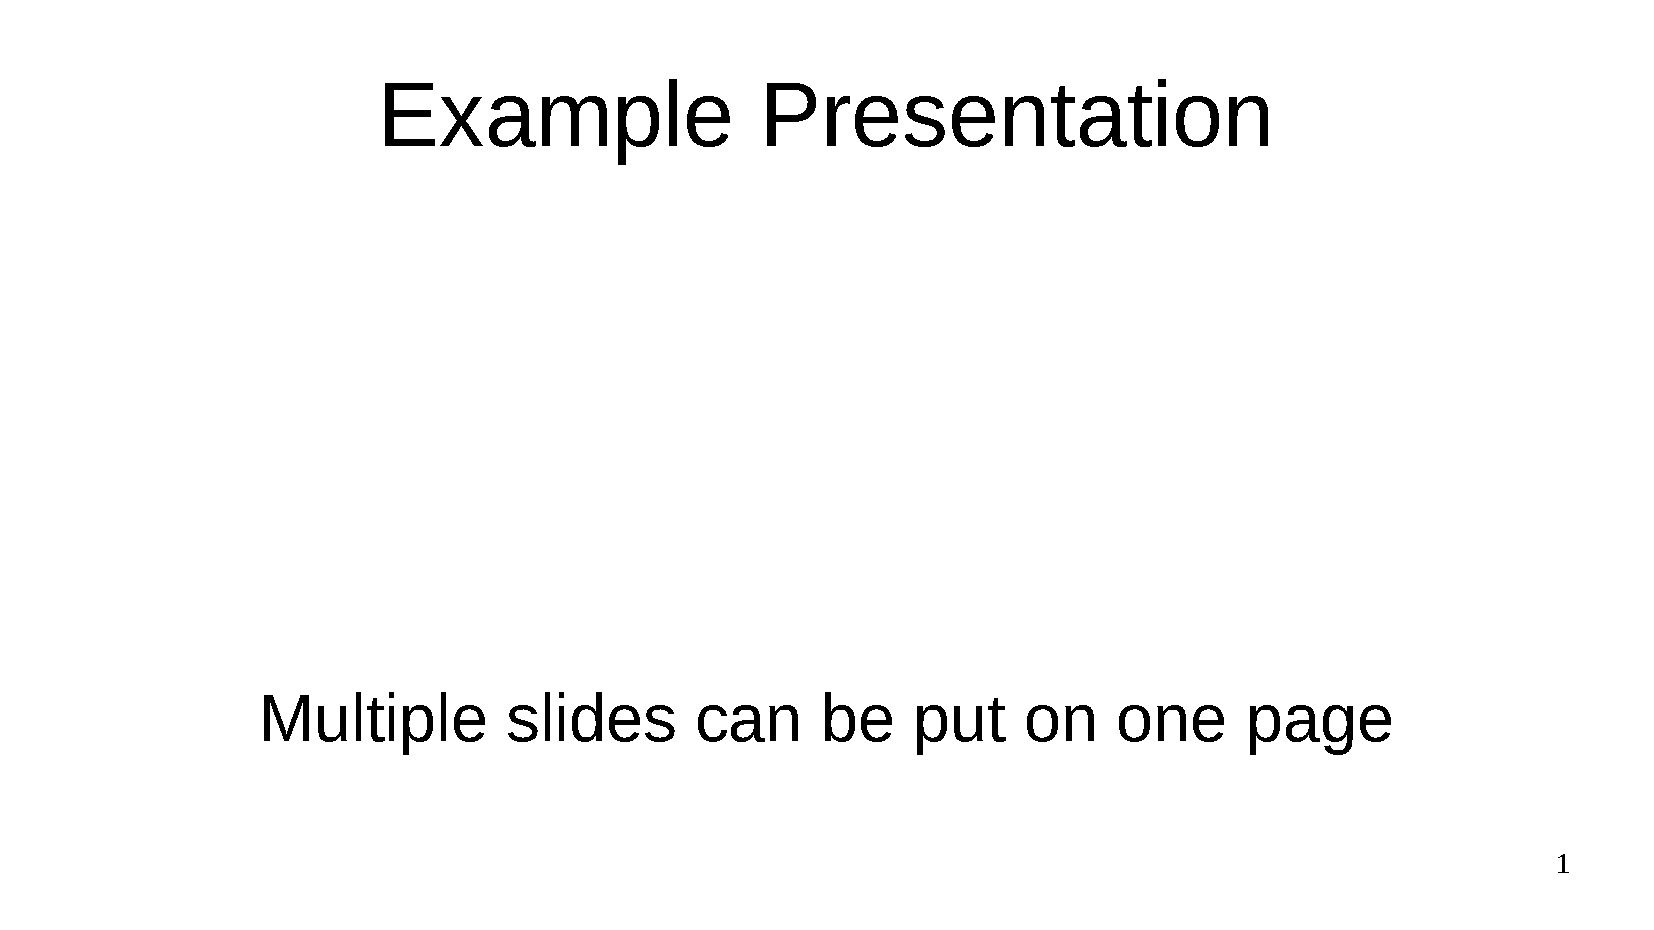
\includepdf[pages=-,nup=1x2,delta=5mm 5mm,landscape=false,pagecommand={}]{pdfs/example-slides.pdf} % chktex 29

\section{Reference}

\subsection{Example}

\begin{itemize}
  \item Included image.  It is also possible to include images.
\end{itemize}

\begin{figure}[H]
  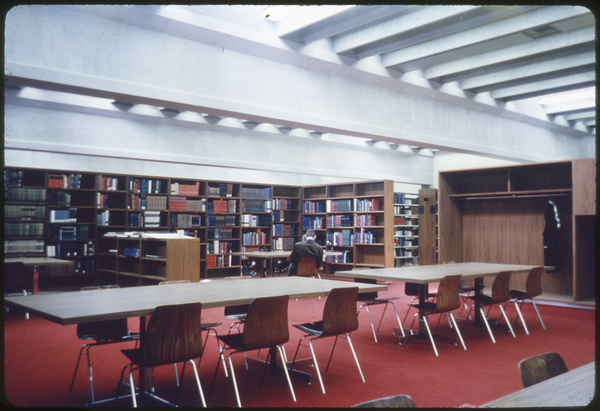
\includegraphics[height=4in]{images/yul 1121686_Medium_sized_JPEG.jpg}
  % \href makes a hyperlink with anchor text.
  \caption{The Steacie Science Library in 1965. \\ \href{https://digital.library.yorku.ca/yul-1121686/steacie-science-library-interior-view}{View in YUDL}.}
\end{figure}

\newpage

\renewcommand\thechapter{B}
\chapter{Professional Contributions and Standing}

\section{Publications}

\subsection{``Article Title'' (\textit{Journal Title})}

% Note that "quotes" won't look fancy.  You need to use ``two single quotes''.  That's just how LaTeX works.

(Do not include the article itself.  Use the citation, which could look like this.)

% Ampersands need to have a backslash in front of them.

Wakaruk, Amanda, Céline Gareau-Brennan, and Matthew Pietrosanu. ``Introducing the Copyright Anxiety Scale.'' \textit{Journal of Copyright in Education \& Librarianship} 5, no. 1 (September 2021). \url{https://doi.org/10.17161/jcel.v5i1.15212}.

\vspace{\baselineskip}

\committeenote{A note from the committee can be added with {\tt committeenote}, where necessary.  It is in italics.

  This can be used to include the brief collaborator statements about the candidate's contributions.

  One co-author said, ``The candidate did A, B and C.''

  Another co-author said, ``The candidate contributed to sections X and Y.''

}

\newpage

\section{Presentations and talks}

\subsection{``Title of Talk'' (Conference, 2023)}

\begin{itemize}
  \item Slides from talk.
\end{itemize}

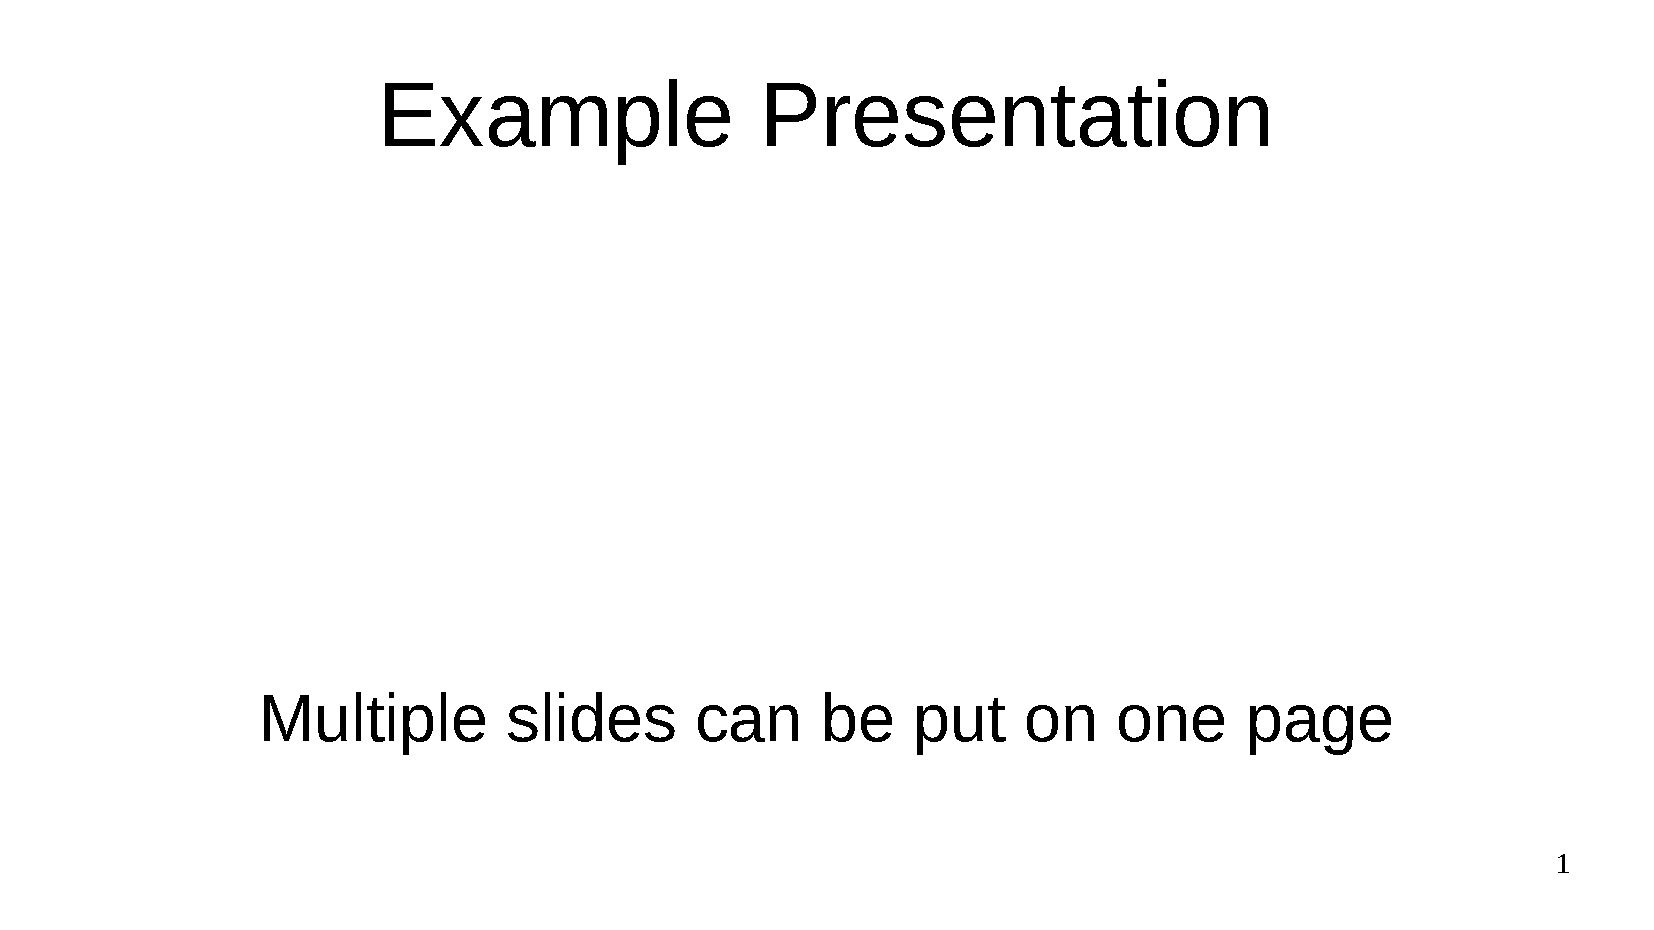
\includepdf[pages=-,nup=2x3,delta=5mm 5mm,landscape=false,pagecommand={}]{pdfs/example-slides.pdf} % chktex 29

\section{Professional Associations}

\subsection{Association name}

\begin{itemize}
  \item Included PDF described here.
\end{itemize}

\candidatenote{
  This is a note from the candidate.  It has a different typeface and stands out from the rest of the file.
}


\includepdf[pages=-,scale=0.95,pagecommand={}]{pdfs/example-1.pdf}

\renewcommand\thechapter{C}
\chapter{Service}

\section{York University Libraries}

\subsection{Library Committee}

\begin{itemize}
  \item The annual report of the committee.  PDFs can be included in landscape view, which has a different orientation on screen but should print normally.
\end{itemize}


\includepdf[pages=-,landscape=true,scale=0.95,pagecommand={}]{pdfs/example-1-landscape.pdf}

\section{York University}

\subsection{University Committee}

\begin{itemize}
  \item The annual report of the committee.
\end{itemize}

\committeenote{The FPC might need to add a brief note explaining that most of the work of a committee is confidential in nature.}

\candidatenote{A candidate's note can go on the same page as a committee note.

It can have two paragraphs and \textit{text in italics}.}


\includepdf[pages=-,scale=0.95,pagecommand={}]{pdfs/example-1.pdf}

\end{document}
